\section{簡単な使い方}

\begin{frame}[fragile]{手順 1/4\\「提案ツールのソースコードを取得する」}
    提案ツールの\href{https://github.com/posl/dit}{\textcolor{teal!60}{リポジトリ}}をクローンする.
    \vskip2.0zh

    実行例
\begin{lstlisting}[]
URL=https://github.com/posl/dit.git
git clone --depth 1 "${URL}"
\end{lstlisting}

\end{frame}


\begin{frame}{手順 2/4\\「開発用のコンテナを起動し,開発を開始する」}
    \vskip0.5zh
    ルートにある,\textcolor{orange}{exec.sh}というシェルスクリプトを実行する.
    \vskip0.5zh

    \begin{figure}
        \centering
        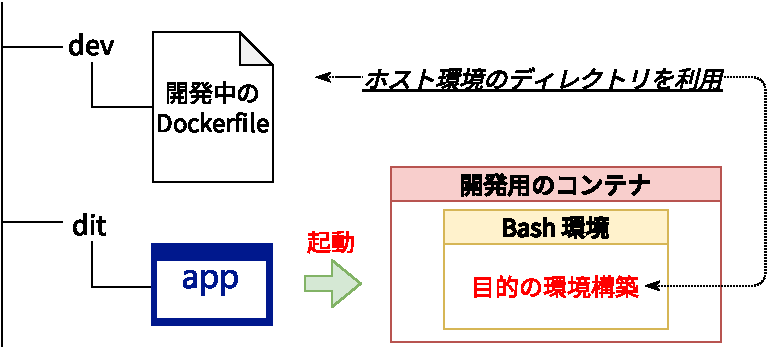
\includegraphics[width=\linewidth]{img/usage1.pdf}
    \end{figure}
\end{frame}


\begin{frame}{手順 3/4\\「動作確認しながら,目的の環境構築を行う」}
    \vskip1.0zh
    動作確認に専念しながら,\textcolor{orange}{対話的に}Dockerfileを開発する.
    \vskip1.0zh

    \begin{figure}
        \centering
        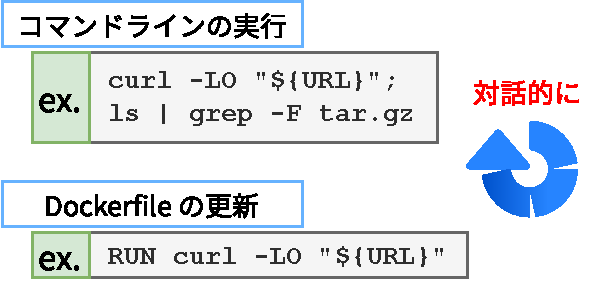
\includegraphics[width=\linewidth]{img/usage2.pdf}
    \end{figure}
\end{frame}


\begin{frame}{手順 4/4\\「Dockerfileを完成させる」}
    次の処理は,提案ツールの機能を使う.
    \begin{description}[labelwidth=6.0zw]
        \item[dit package] パッケージのインストール
        \item[dit copy] ホスト環境からのファイルのコピー
        \item[dit optimize] Dockerfileのリファクタリング・最適化
    \end{description}

    \vskip2.0zh
    最後に,Dockerfileのリファクタリング・最適化を行う.
\end{frame}